\documentclass{beamer}
\usetheme{Madrid}

\title{Feedback Vertex Set with Bounded Cycle Length: Approximation, Tractability and Beyond the Worst-Case Analysis}
\author{Martin Sokolov}
\institute{Utrecht University}
\date{\today}

\usepackage{tikz}
\usepackage{tikz-qtree}
\usetikzlibrary{positioning, shapes, trees}
\usetikzlibrary{backgrounds}

\usepackage{algorithm}
\usepackage{algorithmic}
\usepackage{amsthm}
\usepackage{amssymb}
\usepackage{longtable}
\usepackage{caption}
\usepackage{graphicx}
\usepackage{adjustbox}
\usepackage{array}
\usepackage{booktabs}

\usetikzlibrary{positioning}

\newcommand{\tw}{\operatorname{tw}}
\newtheorem{result}{Result}

\begin{document}

\begin{frame}
  \titlepage
\end{frame}

\begin{frame}{Outline}
  \tableofcontents
\end{frame}

\section{Problem Overview}

\begin{frame}{Problems Studied (Emphasis on Focus Areas)}

\begin{itemize}
    \item Dominating Set
    \item \textcolor{red!50}{Feedback Vertex Set (FVS)}
    \item \textcolor{red}{Feedback Vertex Set with Four Cycle Length (FVS-4CL)}
    \item \textcolor{red}{Feedback Vertex Set with Bounded Cycle Length (FVS-BCL)}
    \item $r$-Dominating Set ($r$-DS)
\end{itemize}

\vspace{1em}
\small
\textcolor{red}{\textbf{FVS-4CL}} is the primary focus of this work.\\
We aim to generalize results to \textcolor{red}{\textbf{FVS-BCL}}.\\
(Our hope in the beginning was generalizing our results to \textcolor{red!50}{\textbf{FVS}}).
\end{frame}

\begin{frame}{Approximation Algorithms for Feedback Vertex Set (FVS)}

\begin{itemize}
    \item \textbf{$\min\{2\Delta^2,\ 4 \log n\}$ where $\Delta$ is the max. degree in $G$. (Bar-Yehuda et al., 1994)}\\
    \small Primal-dual algorithm on undirected graphs with general vertex weights.

    \item \textbf{2-Approximation (Bafna et al., 1995)}\\
    \small Local ratio technique with improved efficiency.
    
    \item \textbf{2-Approximation (Becker and Geiger, 1996)}\\
    \small Greedy-like approximation algorithm.

    \item \textbf{2-Approximation (Chudak et al., 1998)}\\
    \small A primal-dual algorithm.
    
\end{itemize}

\begin{itemize}
  \item \textbf{Hardness: APX-Complete (Dinur and Safra, 2005)}\\
    \small NP-hard to approximate within a factor better than 1.36 via reduction from Vertex Cover.
\end{itemize}

\end{frame}

\begin{frame}{Approximation Algorithms for Feedback Vertex Set (FVS) in planar graphs}

\begin{itemize}
    \item \textbf{PTAS for FVS (Kleinberg and Kumar, 2001)}
    \item \textbf{PTAS for FVS (Le and Zheng, 2020)}\\
    \small Using a local search heuristic
    \item \textbf{EPTAS for unweighted FVS (Demaine and Hajiaghayi)}\\
    \small Using bidimensionality
    \item \textbf{PTAS for weighted FVS (Cohen-Addad et al., 2016)}\\
    \small Reduction from weighted feedback vertex set
 to vertex-weighted connected dominating set
    \item \textbf{EPTAS for weighted FVS (\textcolor{red}{Open question.})}
\end{itemize}

\end{frame}

\begin{frame}{FVS with Bounded Cycle Length (FVS-BCL)}
  \begin{itemize}
    \item \textbf{Inapproximability of Feedback Vertex Set for Bounded Length Cycles 
    (Guruswami and Lee, 2014)}\\
    \small For any integer constant $\rho \geq 3$ and $\epsilon > 0$, it is
    hard to find a $(\rho-1-\epsilon)$-approximate solution to the problem of intersecting every cycle
    of length at most $\rho$. 
  \end{itemize}
\end{frame}

\section{Approximation Schemes}

\begin{frame}{EPTAS via Baker's Technique}
  We obtain:
  \begin{itemize}
    \item $(1 + 2\epsilon)$-approximation algorithm for the FVS-4CL problem
    
    with a running time of $2^{\mathcal{O}(\tw^2)} \cdot n^{\mathcal{O}(1)}$.
    \item \(\left(1 + \frac{\lfloor\rho/2\rfloor}{\epsilon}\right)\)-approximation for the FVS-BCL problem 
    
    with a running time of \( f\left(\tw, \rho\right) \cdot n^{\mathcal{O}\left(1\right)} \) 
    for some computable function $f$.
  \end{itemize}
\end{frame}

\begin{frame}[fragile]{Baker's Technique for Unweighted FVS-4CL}
\small % reduce font size to fit more text nicely
    \begin{algorithm}[H]
        \caption{Baker's technique for the unweighted FVS-4CL}
        \label{alg:unweighted_feedback_vertex_set_global}
        \begin{algorithmic}[1]
        \REQUIRE Planar graph $G = (V, E)$, parameter $\ell \leftarrow \frac{1}{\epsilon}$
        \ENSURE $(1 + \epsilon)$-approximation for \textsc{FVS-4CL}
        \STATE Perform \textsc{BFS} from some arbitrary vertex $r$ \label{alg3:line1}
        \STATE $S \leftarrow \emptyset$

        $i$: \textit{shift}; $j$: \textit{slice}

        \FOR{each $i = 0$ to $\ell-1$} \label{alg3:for-loop}
            \STATE Let $G_{i, j}$ be the subgraph induced on vertices at levels
            $j \cdot \ell + i$ through $(j+1) \cdot \ell + i + 1$ for all $j \geq 0$. \label{alg3:line4}
            \STATE Let $S_{i, j}$ be the minimum unweighted \textsc{FVS-4CL} of $G_{i, j}$ using Algorithm~\ref{alg:dp} as a subroutine (weights are all ones). \label{alg3:subroutine}
            \STATE Let $S_i = \bigcup_{j} S_{i, j}$ \label{alg3:line6}
            \STATE $S \leftarrow S \cup \{S_i\}$ \label{alg3:line7}
        \ENDFOR
        \RETURN $S_{i^*}$ from $S$ with minimum cardinality \label{alg3:line9}
        \end{algorithmic}
    \end{algorithm}
\end{frame}

\begin{frame}{BFS Layered Tree Structure}
    \begin{columns}

        \begin{column}{0.40\textwidth}
            \textbf{Idea:} Break graph into layers via BFS. \\
            \vspace{1em}
            \begin{itemize}
                \item Nodes grouped by distance from root.
                \item Overlap grouped by distance from root $\mod \ell$ 
                \item Subgraphs $G_{0,0}, G_{0,1}, G_{0,2}, \dots$ 
            \end{itemize}
        \end{column}

        \begin{column}{0.60\textwidth}
            \centering
            \resizebox{\textwidth}{!}{%
                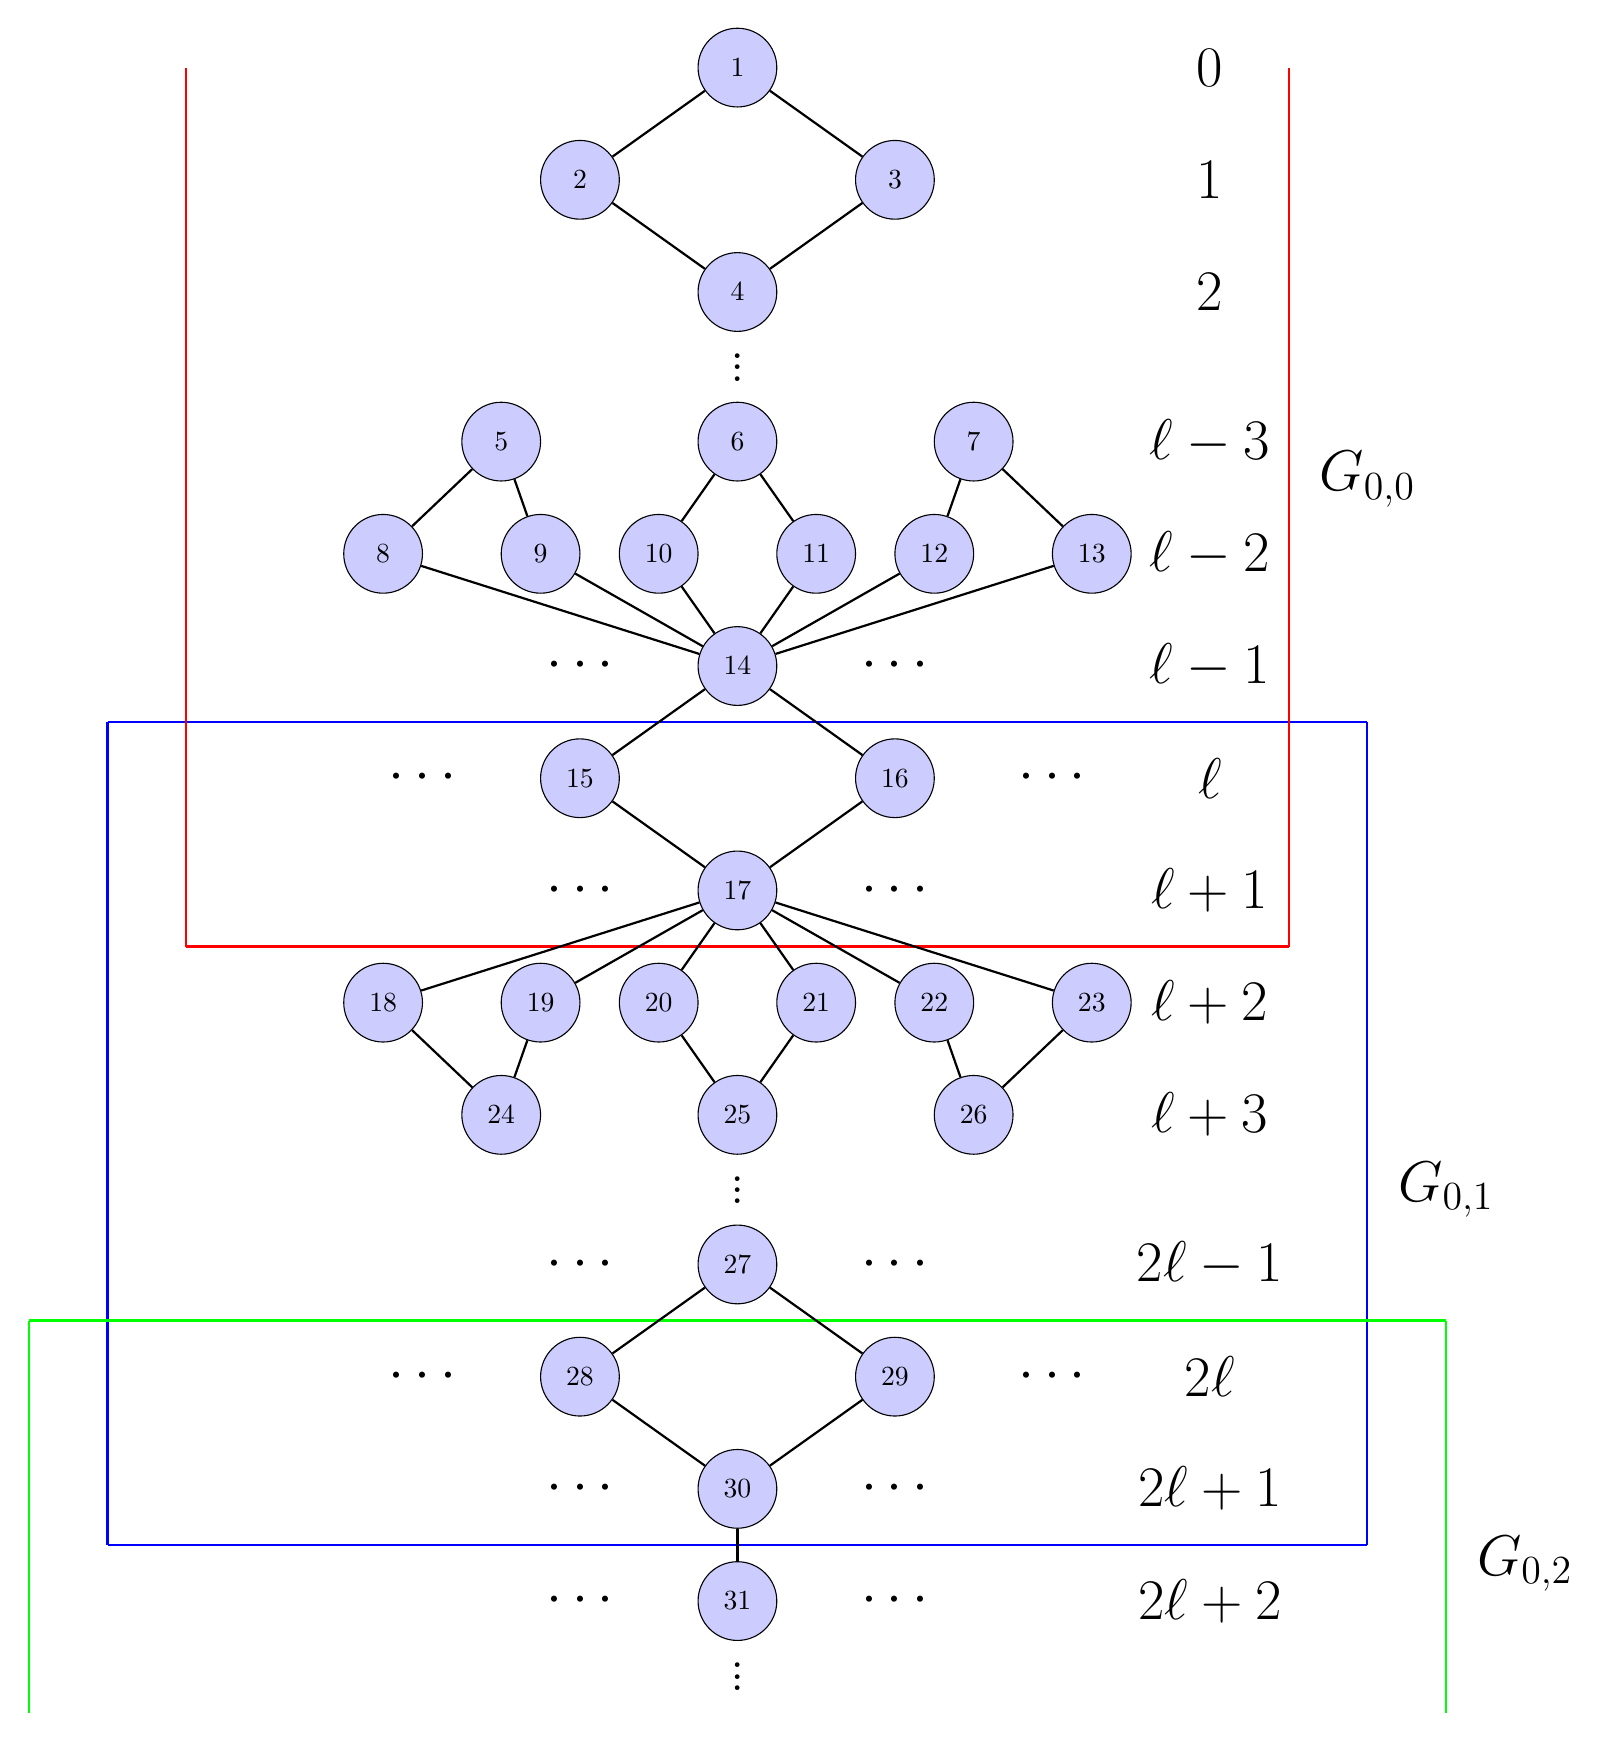
\begin{tikzpicture}[yscale=0.95]
                    % Level 0 (Root node)
                    \node[circle, draw, fill=blue!20, minimum size=10mm] (1) at (0, 0) {1};

                    % Level 1
                    \node[circle, draw, fill=blue!20, minimum size=10mm] (2) at (-2, -1.5) {2};
                    \node[circle, draw, fill=blue!20, minimum size=10mm] (3) at (2, -1.5) {3};

                    % Level 2
                    \node[circle, draw, fill=blue!20, minimum size=10mm] (4) at (0, -3) {4};

                    % Dotted vertical line indicating further levels
                    \node[draw=none] at (0, -3.9) { \huge $\vdots$ };

                    % Level l-3
                    \node[circle, draw, fill=blue!20, minimum size=10mm] (5) at (-3, -5){5};
                    \node[circle, draw, fill=blue!20, minimum size=10mm] (6) at (0, -5) {6};
                    \node[circle, draw, fill=blue!20, minimum size=10mm] (7) at (3, -5) {7};

                    % Level l-2
                    \node[circle, draw, fill=blue!20, minimum size=10mm] (8) at (-4.5, -6.5){8};
                    \node[circle, draw, fill=blue!20, minimum size=10mm] (9) at (-2.5, -6.5) {9};
                    \node[circle, draw, fill=blue!20, minimum size=10mm] (10) at (-1, -6.5) {10};
                    \node[circle, draw, fill=blue!20, minimum size=10mm] (11) at (1, -6.5) {11};
                    \node[circle, draw, fill=blue!20, minimum size=10mm] (12) at (2.5, -6.5) {12};
                    \node[circle, draw, fill=blue!20, minimum size=10mm] (13) at (4.5, -6.5) {13};
                    
                    % Level l-1
                    \node[circle, draw, fill=blue!20, minimum size=10mm] (14) at (0, -8){14};

                    \node[draw=none] at (2, -8) {\huge $\cdots$};
                    \node[draw=none] at (-2, -8) {\huge $\cdots$};

                    % Vertical line between levels l-1 and l
                    \draw[thick, blue] (-8, -8.75) -- (8, -8.75);
                    \draw[thick, blue] (-8, -8.75) -- (-8, -19.75);
                    \draw[thick, blue] (8, -8.75) -- (8, -19.75);
                    \draw[thick, blue] (-8, -19.75) -- (8, -19.75);
                    \node[draw=none] at (9, -15) {\huge $G_{0, 1}$};

                    % Level l
                    \node[circle, draw, fill=blue!20, minimum size=10mm] (15) at (-2, -9.5){15};
                    \node[circle, draw, fill=blue!20, minimum size=10mm] (16) at (2, -9.5){16};

                    \node[draw=none] at (4, -9.5) {\huge $\cdots$};
                    \node[draw=none] at (-4, -9.5) {\huge $\cdots$};

                    % Level l+1
                    \node[circle, draw, fill=blue!20, minimum size=10mm] (17) at (0, -11){17};
                    
                    % Vertical line between levels l+1 and l+2
                    \draw[thick, red] (-7, -11.75) -- (7, -11.75);
                    \draw[thick, red] (-7, -11.75) -- (-7, 0);
                    \draw[thick, red] (7, -11.75) -- (7, 0);
                    \node[draw=none] at (8, -5.5) {\huge $G_{0, 0}$};

                    % Horizontal dots on level l+1
                    \node[draw=none] at (2, -11) {\huge $\cdots$};
                    \node[draw=none] at (-2, -11) {\huge $\cdots$};

                    % Level l+2
                    \node[circle, draw, fill=blue!20, minimum size=10mm] (18) at (-4.5, -12.5){18};
                    \node[circle, draw, fill=blue!20, minimum size=10mm] (19) at (-2.5, -12.5) {19};
                    \node[circle, draw, fill=blue!20, minimum size=10mm] (20) at (-1, -12.5) {20};
                    \node[circle, draw, fill=blue!20, minimum size=10mm] (21) at (1, -12.5) {21};
                    \node[circle, draw, fill=blue!20, minimum size=10mm] (22) at (2.5, -12.5) {22};
                    \node[circle, draw, fill=blue!20, minimum size=10mm] (23) at (4.5, -12.5) {23};
                    
                    % Level l+3
                    \node[circle, draw, fill=blue!20, minimum size=10mm] (24) at (-3, -14){24};
                    \node[circle, draw, fill=blue!20, minimum size=10mm] (25) at (0, -14) {25};
                    \node[circle, draw, fill=blue!20, minimum size=10mm] (26) at (3, -14) {26};

                    % Dotted vertical line indicating further levels
                    \node[draw=none] at (0, -14.9) { \huge $\vdots$ };

                    % Level 2l - 1
                    \node[circle, draw, fill=blue!20, minimum size=10mm] (27) at (0, -16) {27};

                    \node[draw=none] at (2, -16) {\huge $\cdots$};
                    \node[draw=none] at (-2, -16) {\huge $\cdots$};

                    % Vertical line between levels l+1 and l+2
                    \draw[thick, green] (-9, -16.75) -- (9, -16.75);
                    \draw[thick, green] (-9, -16.75) -- (-9, -22);
                    \draw[thick, green] (9, -16.75) -- (9, -22);

                    % Level 2l
                    \node[circle, draw, fill=blue!20, minimum size=10mm] (28) at (-2, -17.5) {28};
                    \node[circle, draw, fill=blue!20, minimum size=10mm] (29) at (2, -17.5) {29};
                    
                    \node[draw=none] at (4, -17.5) {\huge $\cdots$};
                    \node[draw=none] at (-4, -17.5) {\huge $\cdots$};

                    % Level 2l+1
                    \node[circle, draw, fill=blue!20, minimum size=10mm] (30) at (0, -19) {30};

                    \node[draw=none] at (2, -19) {\huge $\cdots$};
                    \node[draw=none] at (-2, -19) {\huge $\cdots$};

                    % Level 2l+2
                    \node[circle, draw, fill=blue!20, minimum size=10mm] (31) at (0, -20.5) {31};

                    \node[draw=none] at (2, -20.5) {\huge $\cdots$};
                    \node[draw=none] at (-2, -20.5) {\huge $\cdots$};

                    % Dotted vertical line indicating further levels
                    \node[draw=none] at (0, -21.4) { \huge $\vdots$ };

                    \node[draw=none] at (10, -20) {\huge $G_{0, 2}$};


                    % Draw edges for BFS with renumbered vertices
                    \foreach \I/\j in {1/2, 1/3, 2/4, 3/4, 5/8, 5/9, 8/14, 9/14, 6/10, 6/11, 10/14, 11/14,
                    7/12, 7/13, 12/14, 13/14, 14/15, 14/16, 15/17, 16/17, 17/18, 17/19, 17/20, 17/21, 17/22, 17/23,
                    18/24, 19/24, 20/25, 21/25, 22/26, 23/26, 27/28, 27/29, 28/30, 29/30, 30/31}
                        \draw[thick] (\I) -- (\j);

                    \node[draw=none] at (6, 0) {\huge 0};
                    \node[draw=none] at (6, -1.5) {\huge 1};
                    \node[draw=none] at (6, -3) {\huge 2};

                    \node[draw=none] at (6, -5) {\huge $\ell-3$};
                    \node[draw=none] at (6, -6.5) {\huge $\ell-2$};
                    \node[draw=none] at (6, -8) {\huge $\ell-1$};
                    \node[draw=none] at (6, -9.5) {\huge $\ell$};
                    \node[draw=none] at (6, -11) {\huge $\ell+1$};
                    \node[draw=none] at (6, -12.5) {\huge $\ell+2$};
                    \node[draw=none] at (6, -14) {\huge $\ell+3$};

                    \node[draw=none] at (6, -16) {\huge $2\ell-1$};
                    \node[draw=none] at (6, -17.5) {\huge $2\ell$};
                    \node[draw=none] at (6, -19) {\huge $2\ell+1$};

                    \node[draw=none] at (6, -20.5) {\huge $2\ell+2$};
                \end{tikzpicture}
            }
        \end{column}
    \end{columns}
\end{frame}

\begin{frame}{Bounds on the Optimum Solution (Unweighted Case)}
    \footnotesize
    \begin{lemma}[Bound on the Optimum Solution in Subgraphs]
    \label{lemma:opt-unweighted-fvs-4cl}

    Let \( S_{i,j} \) be the minimum unweighted feedback vertex set (FVS-4CL)
    for subgraph \( G_{i,j} \), computed using 
    Algorithm~\ref{alg:unweighted_feedback_vertex_set_global}, and let 
    \( F \equiv \text{OPT} \) be the optimum solution for the full graph \( G \).

    Define \( F_{i,j} := F \cap V(G_{i,j}) \), i.e., the restriction of the global solution \( F \) to the subgraph \( G_{i,j} \).

    Then:
    \[
    |S_{i,j}| \leq |F_{i,j}|
    \]
    \end{lemma}

    \begin{result}[Optimum solution bound for the whole graph]
    \label{result-two}

    Let \( S_i \) be the union of optimal solutions defined on Line~\ref{alg3:line6} of Algorithm~\ref{alg:unweighted_feedback_vertex_set_global} 
    for some shift \( i \). 
    Let \( F \equiv \text{OPT} \) be the optimum solution in \( G \) and let \( F_{i,j} = G_{i,j} \cap F \).
    For those sets it holds that:
    \[
    |S_i| \leq \sum_j |S_{i,j}| \leq \sum_j |F_{i,j}|
    \]
    \end{result}

\end{frame}

\begin{frame}{Bounds on the Optimum Solution (Unweighted Case)}
    \footnotesize
    \begin{lemma}[Bound for the vertices on the boundaries (Unweighted Case)]
        \label{lemma-two}

        Let $F_i = F \cap \{\text{vertices at levels } i \bmod \ell\}$. 
        The sets $F_i$ are disjoint and $\bigcup_i F_i = F$.

        We claim that:
        \[
            \exists q \in \{0, 1, \dots, \ell-1\} : |F_q| + |F_{q+1}| \leq \frac{2}{\ell} \cdot |F| \text{.}
        \]
    \end{lemma}

    \begin{lemma}[Bound for the cardinality of the intersection sets]
    \label{lemma-three}
    Let \( F \equiv \text{OPT} \) be the optimal solution and \( F_{i,j} = F \cap G_{i,j} \) be the intersection 
    sets with the subgraphs. Then we have: 
    \[
    \sum_j |F_{i^*, j}| \leq |F| + \frac{2}{\ell} \cdot |F|
    \]
    for some specific integer \( i^* \).
    \end{lemma}

    \[
    |S_{i^*}| \leq \sum\limits_{j} |S_{i^*, j}| \leq \sum\limits_{j} |F_{i^*, j}| \leq |F| + \frac{2}{\ell} \cdot |F| = (1 + \frac{2}{\ell}) \cdot |F|
    \]

\end{frame}

\begin{frame}{Weighted Bounds for FVS-BCL Problems}

\textbf{Weighted FVS-4CL:}
\[
w(S_{i^*}) \leq \sum\limits_j w(S_{i^*, j}) \leq \sum\limits_j w(F_{i^*, j}) \leq w(F) + \frac{2}{\ell} \cdot w(F) = \left(1 + \frac{2}{\ell}\right) \cdot w(F)
\]

\vspace{1em}

\textbf{Weighted FVS-BCL (break cycles of length $\rho$):}
\[
w(S_{i^*}) \leq \sum\limits_j w(S_{i^*, j}) \leq \sum\limits_j w(F_{i^*, j}) \leq \left(1 + \frac{\lfloor\rho/2\rfloor}{\ell}\right) \cdot w(F)
\]

\end{frame}

\section{Fixed-Parameter Tractability of FVS-BCL}

\begin{frame}
  \centering
  \vfill
  \LARGE \textbf{Fixed-Parameter Tractability of FVS-BCL}
  \vfill
\end{frame}


\begin{frame}{Fixed-Parameter Tractability of FVS-BCL}
  \begin{itemize}
    \item Monadic Second Order Logic for FVS-BCL
    \item Dynamic Programming Algorithm for FVS-BCL using Nice Tree Decompositions
  \end{itemize}
\end{frame}

\begin{frame}{MSOL Formulation}
  \begin{itemize}
    \item An extension of First-Order Logic
    \item Object variables: \textit{vertices}: $v_1, v_2, \dots$ and \textit{edges}: $e_1, e_2, \dots$. 
    \item Set variables: sets of vertices $V_1, V_2, \dots$ and sets of edges $E_1, E_2, \dots$.
    \item Binary relation $\in : \{\text{object variable}\} \times \{\text{set variable}\} \to \{0, 1\}$. Therefore 
    $v \in V$ \textit{iff} $v$ is an element of the corresponding set $V$.
    \item The $Adj(e, v_i, v_j)$ relation. It detects whether edge $e$ is an edge from vertex $v_i$ to 
    vertex $v_j$ where $v_i \neq v_j$.
    \item Quantification over set variables: $\forall V_i, \forall E_i$ and $\exists V_i, \exists E_i$.
  \end{itemize}
\end{frame}

\begin{frame}{MSOL Formulation: Unweighted FVS-4CL}

\begin{equation}
    \label{courcelle:unweighted}
    \begin{aligned}
        \min_{F \subseteq V} & \ |F|: \\
        & \forall v : \forall u : \forall w : \forall z : \\
        & v \in (V \backslash F) \land u \in (V \backslash F) \land w \in (V \backslash F) \land z \in (V \backslash F) \\
        & \land v \neq w \land u \neq z \\
        & \land \neg ((v, u) \in E \land (u, w) \in E \land (w, z) \in E \land (v, z) \in E)
    \end{aligned}
\end{equation}

\end{frame}

\begin{frame}{MSOL Formulation: Weighted FVS-4CL}

\begin{equation}
    \label{courcelle:weighted}
    \begin{aligned}
        \min_{F \subseteq V} & \ w(F): \\
        & \forall v : \forall u : \forall w : \forall z : \\
        & v \in (V \backslash F) \land u \in (V \backslash F) \land w \in (V \backslash F) \land z \in (V \backslash F) \\
        & \land v \neq w \land u \neq z \\
        & \land \neg((v, u) \in E \land (u, w) \in E \land (w, z) \in E \land (v, z) \in E)
    \end{aligned}
\end{equation}

\end{frame}

\begin{frame}{MSOL Formulation: Weighted FVS-$\rho$CL}

\begin{equation}
    \label{courcelle:rho}
    \begin{aligned}
        \min_{F \subseteq V} & \ w(F) : \\
        & \forall v_1 : \forall v_2 : \dots \forall v_{\rho} : \\
        & v_1 \in (V \backslash F) \land v_2 \in (V \backslash F) \dots \land v_{\rho} \in (V \backslash F) \\
        & \land (v_1 \neq v_2 \land v_1 \neq v_3 \land \dots \land v_1 \neq v_{\rho}) \\
        & \land (v_2 \neq v_1 \land v_2 \neq v_3 \land \dots \land v_2 \neq v_{\rho}) \\
        & \dots \\
        & \land (v_{\rho} \neq v_1 \land v_{\rho} \neq v_2 \land \dots \land v_{\rho} \neq v_{\rho-1}) \\
        & \land \neg((v_1, v_2) \in E \land (v_2, v_3) \in E \land \dots \land (v_{\rho-1},v_{\rho}) \in E \land (v_{\rho}, v_1) \in E)
    \end{aligned}
\end{equation}

\end{frame}

\begin{frame}{Courcelle's Theorem and MSOL Solvability of FVS-$\rho$CL}
\footnotesize

\begin{theorem}[Courcelle's theorem]
\label{theorem:courcelle}
Assume that $\phi$ is a MSOL formula and $G$ is an $n$-vertex graph, with an evaluation 
of all free variables of $\phi$. Suppose a tree decomposition of $G$ of width $t$ is given. 
Then there exists an algorithm that verifies whether $\phi$ is satisfied in $G$ in time:
\[
    f(\|\phi\|, t) \cdot n^{\mathcal{O}(1)}
\]
for some computable function $f$.
\end{theorem}

\begin{corollary}[MSOL Solvability of FVS-$\rho$CL on Bounded-Treewidth Graphs]
\label{cor:msol-fvs-rho}
Let $\rho \ge 3$ be a constant and $G = (V,E)$ be a graph of treewidth at most $\tw$, with vertex-weight function $w : V \to \mathbb{N}$.
Then the minimum-weight set breaking all $\rho$-cycles (FVS-$\rho$CL) can be computed in time:
\[
    f(\rho, \tw) \cdot n^{\mathcal{O}(1)}
\]
for some computable function $f$ depending only on $\rho$ and $\tw$.
\end{corollary}

\end{frame}

\begin{frame}
  \centering
  \vfill
  \LARGE \textbf{Dynamic Programming Algorithm for FVS-4CL over Nice Tree Decompositions}
  \vfill
\end{frame}

\begin{frame}{Algorithm Design for FVS-4CL}
\footnotesize
\begin{enumerate}
    \item \textbf{Solution:} For the FVS-4CL problem, a solution for graph \(G\) is a set \(F\) such that \(G - F\) contains no 4-cycles.

    \item \textbf{Partial Solution:} For subgraph \(G_i = (V_i, E_i)\), a partial solution \(F_i\) is a subset \(F_i \subseteq V_i\), a restriction of a full solution.

    \item \textbf{Extension of Partial Solution:} A solution \(F\) extends \(F_i\) if \(F \cap V_i = F_i\).

    \item \textbf{Characteristic of a Partial Solution:} For \(X_i\), vertices are partitioned as:
    \begin{itemize}
        \item \(I \subseteq X_i\): vertices in the partial solution.
        \item \(\mathcal{F} \subseteq X_i \times X_i\): pairs \((v,u)\) with a common neighbour \(w \in V_i \setminus X_i\) not in \(F_i\).
    \end{itemize}
    \[
    ch(G_i, F_i) = \big(I, \{(v,u) \in X_i \times X_i : \exists w \in V_i \setminus X_i, (v,w), (u,w) \in E_i, w \notin F_i \}\big)
    \]

    The valuation table \(c[i, I, \mathcal{F}] \in \mathbb{N} \cup \{\infty\}\) gives the minimum weight of partial solution \(F_i\):
    \[
    c[i, I, \mathcal{F}] = \min \{ w(W) : W \text{ is a FVS-4CL of } G_i \land W \cap X_i = I \}
    \]

    \item \textbf{Full Set of Characteristics:} For node \(X_i\), valuations exist for all
    \[
    I \in \{0,1\}^{|X_i|} \quad \text{and} \quad \mathcal{F} \in \{0,1\}^{|X_i \times X_i|}
    \]
    There are at most \(2^{(\tw+1)} \cdot 2^{\binom{\tw+1}{2}} = 2^{\mathcal{O}(\tw^2)}\) entries.
\end{enumerate}

\end{frame}

\begin{frame}{DP Transitions over Tree Decomposition Nodes}
  \small

  \textbf{Leaf Node:} \(X_i = \emptyset\)

  \vspace{-1em}
  \[
  c[i, \emptyset, \emptyset] = 0
  \]

  \textbf{Introduce Node:} 
  Let \( X_i = X_j \cup \{v\} \)

  \vspace{-1em}
  \[
  \begin{aligned}
  c[i, I \cup \{v\}, \mathcal{F}] &= w(v) + c[j, I, \mathcal{F}] \\
  c[i, I, \mathcal{F}] &= 
  \begin{cases}
  \infty & \text{if } \exists u,w \notin I: (u,w) \in \mathcal{F},\ (v,u), (v,w) \in E_i \\
  c[j, I, \mathcal{F}] & \text{otherwise}
  \end{cases}
  \end{aligned}
  \]

  \textbf{Forget Node:}
  Let \( X_i = X_j \setminus \{v\} \)

  \vspace{-0.5em}
  \[
  c[i, I, \mathcal{F}] = \min \left(
  \begin{aligned}
  &c[j, I \cup \{v\}, \mathcal{F}], \\
  &c[j, I, \mathcal{F} \cup \{(u,w) : (v,u), (v,w) \in E_i\}]
  \end{aligned}
  \right)
  \]

  \textbf{Join Node:}
  Let \( X_i = X_{j_1} = X_{j_2} \)

  \vspace{-0.5em}
  \[
  \begin{aligned}
  c[i, I, \mathcal{F}] &= \min_{\mathcal{F}_1 \cup \mathcal{F}_2 = \mathcal{F}} 
  \left( c[j_1, I, \mathcal{F}_1] + c[j_2, I, \mathcal{F}_2] - w(I) \right) \\
  \text{Infeasible if } &\exists u,w \notin I: (u,w) \in \mathcal{F}_1 \cap \mathcal{F}_2 \Rightarrow c[i, I, \mathcal{F}] = \infty
  \end{aligned}
  \]

\end{frame}

\begin{frame}{Rhombus Graph and Tree Decomposition}
  \footnotesize
  \begin{minipage}{0.4\textwidth} % Slightly more space
      \centering
      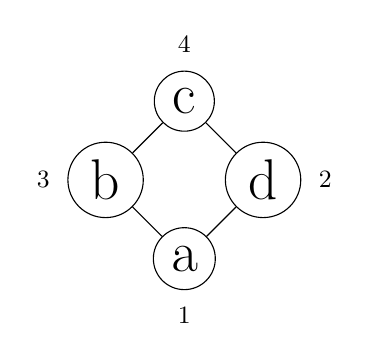
\begin{tikzpicture}
        % Reduced scale and node size to ensure it fits
        \tikzstyle{vertex}=[scale=1, circle, draw, minimum size=10pt] 

        \node[vertex] (a) at (0, 0) {\huge a};
        \node[vertex] (b) at (-1, 1) {\huge b};
        \node[vertex] (c) at (0, 2) {\huge c};
        \node[vertex] (d) at (1, 1) {\huge d};

        \draw (a) -- (b);
        \draw (b) -- (c);
        \draw (c) -- (d);
        \draw (d) -- (a);

        \node[below=0.1cm of a] {\small $1$};
        \node[left=0.1cm of b] {\small $3$};
        \node[above=0.1cm of c] {\small $4$};
        \node[right=0.1cm of d] {\small $2$};
      \end{tikzpicture}
      \vspace{2mm} % Optional space
      \textbf{Rhombus Graph $G$}
  \end{minipage}%
  \begin{minipage}{0.2\textwidth} % Slightly more space
      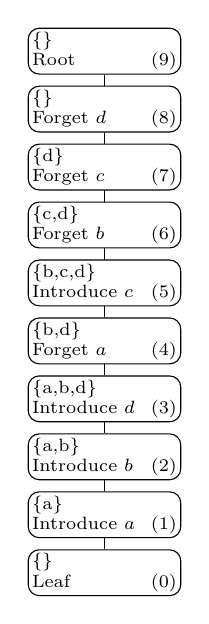
\begin{tikzpicture}[
        every node/.style={
            draw, rounded corners, align=left, 
            font=\scriptsize, 
            text width=2cm, % Reduced text width is the key fix
            inner sep=1.5pt
        }, 
        level distance=0.8cm,
        scale=0.92, transform shape % Slightly reduced scale
      ]
        \node (root) {\{\} \\ Root \hfill (9)}
          child { node (f_d) {\{\} \\ Forget $d$ \hfill (8)}
            child { node (f_c) {\{d\} \\ Forget $c$ \hfill (7)}
              child { node (f_b) {\{c,d\} \\ Forget $b$ \hfill (6)}
                child { node (i_c) {\{b,c,d\} \\ Introduce $c$ \hfill (5)}
                  child { node (f_a) {\{b,d\} \\ Forget $a$ \hfill (4)}
                    child { node (i_d) {\{a,b,d\} \\ Introduce $d$ \hfill (3)}
                      child { node (i_b) {\{a,b\} \\ Introduce $b$ \hfill (2)}
                        child { node (i_a) {\{a\} \\ Introduce $a$ \hfill (1)}
                          child { node (leaf) {\{\} \\ Leaf \hfill (0)} }
                        }
                      }
                    }
                  }
                }
              }
            }
          };
      \end{tikzpicture}
  \end{minipage}%
    \begin{minipage}[c][0.6\textheight][c]{0.45\linewidth} % Container for the title
      \textbf{Nice Tree Decomposition}
      
      of the graph $G$ with a width of 2.
  \end{minipage}
\end{frame}

\begin{frame}{Rhombus Graph and Tree Decomposition}
  \footnotesize
  \begin{minipage}{0.3\textwidth} % Slightly more space
      \centering
      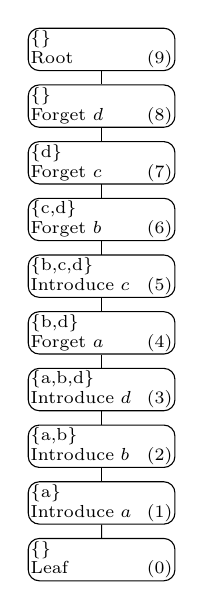
\begin{tikzpicture}[
        every node/.style={
            draw, rounded corners, align=left, 
            font=\scriptsize, 
            text width=2cm, % Reduced text width is the key fix
            inner sep=1pt
        }, 
        level distance=0.8cm,
        scale=0.9, transform shape % Slightly reduced scale
      ]
        \node (root) {\{\} \\ Root \hfill (9)}
          child { node (f_d) {\{\} \\ Forget $d$ \hfill (8)}
            child { node (f_c) {\{d\} \\ Forget $c$ \hfill (7)}
              child { node (f_b) {\{c,d\} \\ Forget $b$ \hfill (6)}
                child { node (i_c) {\{b,c,d\} \\ Introduce $c$ \hfill (5)}
                  child { node (f_a) {\{b,d\} \\ Forget $a$ \hfill (4)}
                    child { node (i_d) {\{a,b,d\} \\ Introduce $d$ \hfill (3)}
                      child { node (i_b) {\{a,b\} \\ Introduce $b$ \hfill (2)}
                        child { node (i_a) {\{a\} \\ Introduce $a$ \hfill (1)}
                          child { node (leaf) {\{\} \\ Leaf \hfill (0)} }
                        }
                      }
                    }
                  }
                }
              }
            }
          };
      \end{tikzpicture}
  \end{minipage}%
  \begin{minipage}{0.35\textwidth}
    \renewcommand{\arraystretch}{0.85}
    \setlength{\tabcolsep}{0.7pt} 
    \begin{tabular}{|c| >{\small}c | >{\small}c | >{\small}c |}
    \hline
    \textbf{\(i\)} & \textbf{\(I\)} & \textbf{\(\mathcal{F}\)} & \textbf{Value} \\
    \hline
    0 & \( \emptyset \) & \( \emptyset \) & 0 \\
    \hline
    % Introduce a
    1 & \( a \) & \( \emptyset \) & 1 \\
    1 & \( \emptyset \) & \( \emptyset \) & 0 \\
    \hline
    % Introduce b
    2 & \( \{ a, b \} \) & \( \emptyset \) & 4 \\
    2 & \( \{ a \} \) & \( \emptyset \) & 1 \\
    2 & \( \{ b \} \) & \( \emptyset \) & 3 \\
    2 & \( \emptyset \) & \( \emptyset \) & 0 \\
    \hline
    % Introduce d
    3 & \( \{ a, b, d \} \) & \( \emptyset \) & 6 \\
    3 & \( \{ a, b \} \) & \( \emptyset \) & 4 \\
    3 & \( \{ a, d \} \) & \( \emptyset \) & 3 \\
    3 & \( \{ b, d \} \) & \( \emptyset \) & 5 \\
    3 & \( \{ a \} \) & \( \emptyset \) & 1 \\
    3 & \( \{ b \} \) & \( \emptyset \) & 3 \\
    3 & \( \{ d \} \) & \( \emptyset \) & 2 \\
    3 & \( \emptyset \) & \( \emptyset \) & 0 \\
    \hline
    % Forget a
    4 & \( \{ b, d \} \) & \( \emptyset \) & 6 \\
    4 & \( \{ b, d \} \) & \( \{ b, d \} \) & 5 \\
    4 & \( \{ b \} \) & \( \emptyset \) & 4 \\
    4 & \( \{ b \} \) & \( \{ b, d \} \) & 3 \\

    \hline
    \end{tabular}
  \end{minipage}
  \begin{minipage}{0.1\textwidth}
    \renewcommand{\arraystretch}{0.5} 
    \setlength{\tabcolsep}{0.7pt} 
    \begin{tabular}{|c| >{\small}c | >{\small}c | >{\small}c |}
    \hline
    \textbf{\(i\)} & \textbf{\(I\)} & \textbf{\(\mathcal{F}\)} & \textbf{Value} \\
    \hline
    4 & \( \{ d \} \) & \( \emptyset \) & 3 \\
    4 & \( \{ d \} \) & \( \{ b, d \} \) & 2 \\
    4 & \( \emptyset \) & \( \emptyset \) & 1 \\
    4 & \( \emptyset \) & \( \{ b, d \} \) & 0 \\
    \hline
        % Introduce c
    5 & \( \{ b, c, d \} \) & \( \emptyset \) & 10 \\
    5 & \( \{ b, c, d \} \) & \( \{ b,d \} \) & 9 \\
    5 & \( \{ b, d \} \) & \( \emptyset \) & 6 \\
    5 & \( \{ b, d \} \) & \( \{ b, d \} \) & 5 \\
    5 & \( \{ b, c \} \) & \( \emptyset \) & 8 \\
    5 & \( \{ b, c \} \) & \( \{ b, d \} \) & 7 \\
    5 & \( \{ b \} \) & \( \emptyset \) & 4 \\
    5 & \( \{ b \} \) & \( \{ b, d \} \) & 3 \\
    5 & \( \{ c, d \} \) & \( \emptyset \) & 7 \\
    5 & \( \{ c, d \} \) & \( \{ b, d \} \) & 6 \\
    5 & \( \{ d \} \) & \( \emptyset \) & 3 \\
    5 & \( \{ d \} \) & \( \{ b, d \} \) & 2 \\
    5 & \( \{ c \} \) & \( \emptyset \) & 5 \\
    5 & \( \{ c \} \) & \( \{ b, d \} \) & 4 \\
    5 & \( \emptyset \) & \( \emptyset \) & 1 \\
    5 & \( \emptyset \) & \( \{ b, d \} \) & \( \infty \) \\
    \hline
    \end{tabular}
  \end{minipage}
\end{frame}

\begin{frame}{Rhombus Graph and Tree Decomposition}
  \footnotesize
  \begin{minipage}{0.3\textwidth} % Slightly more space
      \centering
      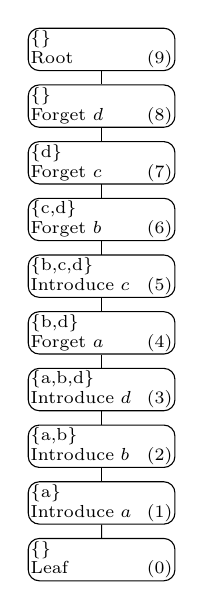
\begin{tikzpicture}[
        every node/.style={
            draw, rounded corners, align=left, 
            font=\scriptsize, 
            text width=2cm, % Reduced text width is the key fix
            inner sep=1pt
        }, 
        level distance=0.8cm,
        scale=0.9, transform shape % Slightly reduced scale
      ]
        \node (root) {\{\} \\ Root \hfill (9)}
          child { node (f_d) {\{\} \\ Forget $d$ \hfill (8)}
            child { node (f_c) {\{d\} \\ Forget $c$ \hfill (7)}
              child { node (f_b) {\{c,d\} \\ Forget $b$ \hfill (6)}
                child { node (i_c) {\{b,c,d\} \\ Introduce $c$ \hfill (5)}
                  child { node (f_a) {\{b,d\} \\ Forget $a$ \hfill (4)}
                    child { node (i_d) {\{a,b,d\} \\ Introduce $d$ \hfill (3)}
                      child { node (i_b) {\{a,b\} \\ Introduce $b$ \hfill (2)}
                        child { node (i_a) {\{a\} \\ Introduce $a$ \hfill (1)}
                          child { node (leaf) {\{\} \\ Leaf \hfill (0)} }
                        }
                      }
                    }
                  }
                }
              }
            }
          };
      \end{tikzpicture}
  \end{minipage}%
  \begin{minipage}{0.35\textwidth}
    \centering
    \renewcommand{\arraystretch}{0.85}
    \setlength{\tabcolsep}{0.7pt} 
    \begin{tabular}{|c| >{\small}c | >{\small}c | >{\small}c |}
    \hline
    \textbf{\(i\)} & \textbf{\(I\)} & \textbf{\(\mathcal{F}\)} & \textbf{Value} \\
    \hline

    6 & \( \{ c, d \} \) & \( \emptyset \) & 10 \\
    6 & \( \{ c, d \} \) & \( \emptyset \) & 9 \\
    6 & \( \{ d \} \) & \( \emptyset \) & 6 \\
    6 & \( \{ d \} \) & \( \emptyset \) & 5 \\

    6 & \( \{ c \} \) & \( \emptyset \) & 8 \\
    6 & \( \{ c \} \) & \( \emptyset \) & 7 \\
    6 & \( \emptyset \) & \( \emptyset \) & 4 \\
    6 & \( \emptyset \) & \( \emptyset \) & 3 \\
    
    6 & \( \{ c, d \} \) & \( \emptyset \) & 7 \\
    6 & \( \{ c, d \} \) & \( \emptyset \) & 6 \\
    6 & \( \{ d \} \) & \( \emptyset \) & 3 \\
    6 & \( \{ d \} \) & \( \emptyset \) & 2 \\

    6 & \( \{ c \} \) & \( \emptyset \) & 5 \\
    6 & \( \{ c \} \) & \( \emptyset \) & 4 \\
    6 & \( \emptyset \) & \( \emptyset \) & 1 \\
    6 & \( \emptyset \) & \( \emptyset \) & \( \infty \) \\

    \hline
    \end{tabular}
  \end{minipage}
  \begin{minipage}{0.1\textwidth}
    \centering
    \renewcommand{\arraystretch}{0.5} 
    \setlength{\tabcolsep}{0.7pt} 
    \begin{tabular}{|c| >{\small}c | >{\small}c | >{\small}c |}
    \hline
    \textbf{\(i\)} & \textbf{\(I\)} & \textbf{\(\mathcal{F}\)} & \textbf{Value} \\
    \hline
    6 & \( \{ c, d \} \) & \( \emptyset \) & 6 \\
    6 & \( \{ d \} \) & \( \emptyset \) & 2 \\
    6 & \( \{ c \} \) & \( \emptyset \) & 4 \\
    6 & \( \emptyset \) & \( \emptyset \) & 1 \\
    \hline
    7 & \( \{ d \} \) & \( \emptyset \) & 2 \\
    7 & \( \emptyset \) & \( \emptyset \) & 1 \\
    \hline
    % Forget d
    8 & \( \emptyset \) & \( \emptyset \) & 1 \\
    \hline
    % Final
    9 & \( \emptyset \) & \( \emptyset \) & 1 \\
    \hline
    \end{tabular}
  \end{minipage}
\end{frame}


\section{Certified Algorithms}

\begin{frame}
  \centering
  \vfill
  \LARGE \textbf{Beyond the Worst-Case Analysis}
  \vfill
\end{frame}

\begin{frame}{Beyond the Worst-Case Analysis}
  \begin{itemize}
    \item Perturbation resilience
    \item $m$-Stitching and $\Pi$-$m$-Stitching
    \item Certified Algorithms
  \end{itemize}
\end{frame}

\begin{frame}{Definitions: $\gamma$-Perturbation and $\gamma$-Stability}
  \begin{definition}[$\gamma$-Perturbation for Vertex-Optimization Problems]
  Let $(G, w)$ be a weighted graph. For any $\gamma \in \mathbb{R}_{\geq 0}$, a \textbf{$\gamma$-perturbation} of the weight function 
  $w : V \to \mathbb{N}$ is a function $w' : V \to \mathbb{R}$ such that:
  \[
  w(v) \leq w'(v) \leq \gamma \cdot w(v) \quad \forall v \in V.
  \]
  \end{definition}
  \vspace{0.5em}
  \begin{definition}[$\gamma$-Stability]
  Let $\Pi$ be a vertex-minimization problem. For any $\gamma \in \mathbb{R}_{\geq 0}$, a weighted graph $(G, w)$ is called a 
  \textbf{$\gamma$-stable instance} of $\Pi$ if it admits a unique optimal solution $S$ that remains optimal under all 
  $\gamma$-perturbations of the weight function $w$.
  \end{definition}
\end{frame}


\begin{frame}{Definition: $m$-stitching}
    \begin{definition}[$m$-stitching]
        \label{m-stitch}
        Assume $m \geq 0$ is an integer, $J$ is an induced subgraph of $G$, and 
        $S_1, S_2 \subseteq V(G)$. Then we define the \textit{$m$-stitch} of $S_2$ onto $S_1$ along 
        $J$ as the set:

        \[
        S_3 := (S_1 \setminus J) \cup (S_2 \cap N^{m}_{G}[J]).
        \]
    \end{definition}
\end{frame}

\begin{frame}{Illustration of $2$-stitching}
\footnotesize
\centering
\begin{tabular}{ccc}
    \begin{minipage}{0.3\textwidth}
        \centering
        % Figure 1
        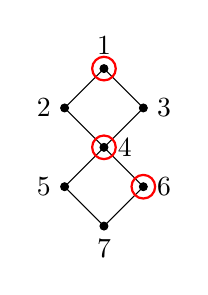
\begin{tikzpicture}[scale=0.5]
            \node[draw, circle, fill=black, scale=0.3, label=above:1] (1) at (0,2) {};
            \node[draw, circle, fill=black, scale=0.3, label=left:2] (2) at (-1,1) {};
            \node[draw, circle, fill=black, scale=0.3, label=right:3] (3) at (1,1) {};
            \node[draw, circle, fill=black, scale=0.3, label=right:4] (4) at (0,0) {};
            \node[draw, circle, fill=black, scale=0.3, label=left:5] (5) at (-1,-1) {};
            \node[draw, circle, fill=black, scale=0.3, label=right:6] (6) at (1,-1) {};
            \node[draw, circle, fill=black, scale=0.3, label=below:7] (7) at (0,-2) {};

            % Draw edges
            \draw (1) -- (2);
            \draw (1) -- (3);
            \draw (2) -- (4);
            \draw (3) -- (4);
            \draw (4) -- (5);
            \draw (4) -- (6);
            \draw (5) -- (7);
            \draw (6) -- (7);

            \draw[red, thick] (1) circle(0.3);
            \draw[red, thick] (4) circle(0.3);
            \draw[red, thick] (6) circle(0.3);
        \end{tikzpicture}
        \captionof{figure}{Vertex set $S_1$}
    \end{minipage}
    &
    \begin{minipage}{0.3\textwidth}
        \centering
        % Figure 2
        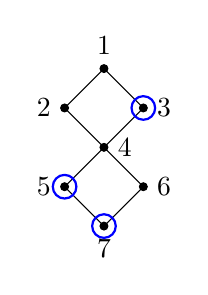
\begin{tikzpicture}[scale=0.5]
            \node[draw, circle, fill=black, scale=0.3, label=above:1] (1) at (0,2) {};
            \node[draw, circle, fill=black, scale=0.3, label=left:2] (2) at (-1,1) {};
            \node[draw, circle, fill=black, scale=0.3, label=right:3] (3) at (1,1) {};
            \node[draw, circle, fill=black, scale=0.3, label=right:4] (4) at (0,0) {};
            \node[draw, circle, fill=black, scale=0.3, label=left:5] (5) at (-1,-1) {};
            \node[draw, circle, fill=black, scale=0.3, label=right:6] (6) at (1,-1) {};
            \node[draw, circle, fill=black, scale=0.3, label=below:7] (7) at (0,-2) {};

            % Draw edges
            \draw (1) -- (2);
            \draw (1) -- (3);
            \draw (2) -- (4);
            \draw (3) -- (4);
            \draw (4) -- (5);
            \draw (4) -- (6);
            \draw (5) -- (7);
            \draw (6) -- (7);

            \draw[blue, thick] (3) circle(0.3);
            \draw[blue, thick] (5) circle(0.3);
            \draw[blue, thick] (7) circle(0.3);
        \end{tikzpicture}
        \captionof{figure}{Vertex set $S_2$}
    \end{minipage}
    &
    \begin{minipage}{0.3\textwidth}
        \centering
        % Figure 3
        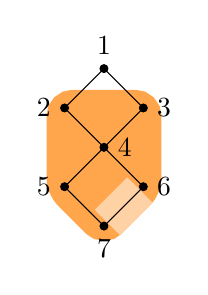
\begin{tikzpicture}[scale=0.5]
            \node[draw, circle, fill=black, scale=0.3, label=above:1] (1) at (0,2) {};
            \node[draw, circle, fill=black, scale=0.3, label=left:2] (2) at (-1,1) {};
            \node[draw, circle, fill=black, scale=0.3, label=right:3] (3) at (1,1) {};
            \node[draw, circle, fill=black, scale=0.3, label=right:4] (4) at (0,0) {};
            \node[draw, circle, fill=black, scale=0.3, label=left:5] (5) at (-1,-1) {};
            \node[draw, circle, fill=black, scale=0.3, label=right:6] (6) at (1,-1) {};
            \node[draw, circle, fill=black, scale=0.3, label=below:7] (7) at (0,-2) {};

            % Draw edges
            \draw (1) -- (2);
            \draw (1) -- (3);
            \draw (2) -- (4);
            \draw (3) -- (4);
            \draw (4) -- (5);
            \draw (4) -- (6);
            \draw (5) -- (7);
            \draw (6) -- (7);

            \begin{scope}[on background layer]
                \filldraw[orange!70,line width=13pt,rounded corners=3pt] (2.center) -- (3.center) -- (6.center) -- (7.center) -- (5.center) -- cycle;
            \end{scope}

            \begin{scope}[on background layer]   
                \filldraw[orange!35,line width=13pt,rounded corners=3pt] (6.center) --  (7.center) -- cycle;
            \end{scope}
        \end{tikzpicture}
        \captionof{figure}{$J$ and $N^2_G[J]$}
    \end{minipage}
    \\
    \begin{minipage}{0.3\textwidth}
        \centering
        % Figure 4
        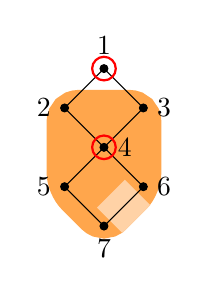
\begin{tikzpicture}[scale=0.5]
            \node[draw, circle, fill=black, scale=0.3, label=above:1] (1) at (0,2) {};
            \node[draw, circle, fill=black, scale=0.3, label=left:2] (2) at (-1,1) {};
            \node[draw, circle, fill=black, scale=0.3, label=right:3] (3) at (1,1) {};
            \node[draw, circle, fill=black, scale=0.3, label=right:4] (4) at (0,0) {};
            \node[draw, circle, fill=black, scale=0.3, label=left:5] (5) at (-1,-1) {};
            \node[draw, circle, fill=black, scale=0.3, label=right:6] (6) at (1,-1) {};
            \node[draw, circle, fill=black, scale=0.3, label=below:7] (7) at (0,-2) {};

            % Draw edges
            \draw (1) -- (2);
            \draw (1) -- (3);
            \draw (2) -- (4);
            \draw (3) -- (4);
            \draw (4) -- (5);
            \draw (4) -- (6);
            \draw (5) -- (7);
            \draw (6) -- (7);

            \begin{scope}[on background layer]   
                \filldraw[orange!70,line width=13pt,rounded corners=5pt] (2.center) -- (3.center) -- (6.center) -- (7.center) -- (5.center) -- cycle;
            \end{scope}

            \begin{scope}[on background layer]   
                \filldraw[orange!35,line width=13pt,rounded corners=5pt] (6.center) --  (7.center) -- cycle;
            \end{scope}

            \draw[red, thick] (1) circle(0.3);
            \draw[red, thick] (4) circle(0.3);

        \end{tikzpicture}
        \captionof{figure}{Remove $J$ from $S_1$}
    \end{minipage}
    &
    \begin{minipage}{0.3\textwidth}
        \centering
        % Figure 5
        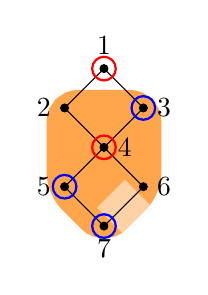
\begin{tikzpicture}[scale=0.5]
            \node[draw, circle, fill=black, scale=0.3, label=above:1] (1) at (0,2) {};
            \node[draw, circle, fill=black, scale=0.3, label=left:2] (2) at (-1,1) {};
            \node[draw, circle, fill=black, scale=0.3, label=right:3] (3) at (1,1) {};
            \node[draw, circle, fill=black, scale=0.3, label=right:4] (4) at (0,0) {};
            \node[draw, circle, fill=black, scale=0.3, label=left:5] (5) at (-1,-1) {};
            \node[draw, circle, fill=black, scale=0.3, label=right:6] (6) at (1,-1) {};
            \node[draw, circle, fill=black, scale=0.3, label=below:7] (7) at (0,-2) {};

            % Draw edges
            \draw (1) -- (2);
            \draw (1) -- (3);
            \draw (2) -- (4);
            \draw (3) -- (4);
            \draw (4) -- (5);
            \draw (4) -- (6);
            \draw (5) -- (7);
            \draw (6) -- (7);

            \begin{scope}[on background layer]   
                \filldraw[orange!70,line width=13pt,rounded corners=5pt] (2.center) -- (3.center) -- (6.center) -- (7.center) -- (5.center) -- cycle;
            \end{scope}

            \begin{scope}[on background layer]   
                \filldraw[orange!35,line width=13pt,rounded corners=5pt] (6.center) --  (7.center) -- cycle;
            \end{scope}

            \draw[red, thick] (1) circle(0.3);
            \draw[red, thick] (4) circle(0.3);

            \draw[blue, thick] (3) circle(0.3);
            \draw[blue, thick] (5) circle(0.3);
            \draw[blue, thick] (7) circle(0.3);
        \end{tikzpicture}
        \captionof{figure}{Add $S_2 \cap N^2_G[J]$}
    \end{minipage}
    &
    \begin{minipage}{0.3\textwidth}
        \centering
        % Figure 6
        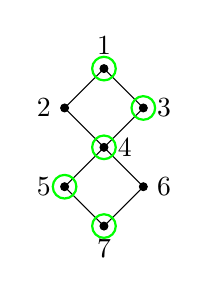
\begin{tikzpicture}[scale=0.5]
            \node[draw, circle, fill=black, scale=0.3, label=above:1] (1) at (0,2) {};
            \node[draw, circle, fill=black, scale=0.3, label=left:2] (2) at (-1,1) {};
            \node[draw, circle, fill=black, scale=0.3, label=right:3] (3) at (1,1) {};
            \node[draw, circle, fill=black, scale=0.3, label=right:4] (4) at (0,0) {};
            \node[draw, circle, fill=black, scale=0.3, label=left:5] (5) at (-1,-1) {};
            \node[draw, circle, fill=black, scale=0.3, label=right:6] (6) at (1,-1) {};
            \node[draw, circle, fill=black, scale=0.3, label=below:7] (7) at (0,-2) {};

            % Draw edges
            \draw (1) -- (2);
            \draw (1) -- (3);
            \draw (2) -- (4);
            \draw (3) -- (4);
            \draw (4) -- (5);
            \draw (4) -- (6);
            \draw (5) -- (7);
            \draw (6) -- (7);

            \draw[green, thick] (1) circle(0.3);
            \draw[green, thick] (3) circle(0.3);
            \draw[green, thick] (4) circle(0.3);
            \draw[green, thick] (5) circle(0.3);
            \draw[green, thick] (7) circle(0.3);

        \end{tikzpicture}
        \captionof{figure}{Final set $S_3$}
    \end{minipage}
\end{tabular}
\end{frame}

\begin{frame}{Meta-Theorem for Minor-Closed Graph Classes}

\begin{theorem}[Meta-Theorem for Minor-Closed Graph Classes]
Let $\mathcal{G}$ be a minor-closed graph class whose local treewidth is bounded by $g(r) = \lambda \cdot r$, for fixed $\lambda \in \mathbb{R}$ and $r \in \mathbb{N}$.

Let $\Pi$ be a vertex-minimization problem such that:
\begin{enumerate}
    \item $\Pi$ is guessable.
    \item $\Pi$ is m-stitchable.
    \item There exists an algorithm $A_\Pi$ that solves $\Pi$-$m$-stitching in time 
    $f(t) \cdot |V(G)|^{\mathcal{O}(1)}$, where $t = \tw(G[N_G^m(J)])$ and $f$ is computable.
\end{enumerate}

Then, for each $\epsilon > 0$, there exists a $(1 + \epsilon)$-certified algorithm for $\Pi$ 
running in time $f(\lambda \cdot m / \epsilon) \cdot |V(G)|^{\mathcal{O}(1)}$ on any input 
$(G, w : V(G) \to \mathbb{N})$, with $G \in \mathcal{G}$ and polynomially-bounded weights.
\end{theorem}

\end{frame}

\begin{frame}{Guessable Problems}
    \begin{definition}[Guessable]
        A problem $\Pi$ is \emph{guessable} if there is an algorithm that outputs a 
        feasible solution 
        with no requirement for optimality in polynomial time.
    \end{definition}

    \textbf{In the case of FVS-BCL}:

    This set is $F \leftarrow V$ for a graph $G = (V, E)$.
\end{frame}

\begin{frame}{Lemma: FVS-BCL is 2-stitchable}
  \begin{lemma}[FVS-BCL is 2-stitchable]
    Let $(G, w)$ be any instance of the FVS-4CL problem, let $J \subseteq V(G)$ be a subset
    of the vertices in the graph, and let $S_1$ and $S_2$ be any two feasible solutions 
    to the problem in $G$. Then the set
    \[
    S_3 := (S_1 \setminus J) \cup (S_2 \cap N^{2}_{G}[J])
    \]
    is a feasible solution to the problem.
  \end{lemma}
\end{frame}

\begin{frame}[fragile]{Stitch-FVS-4CL Algorithm}
  \begin{algorithm}[H]
  \caption{Stitch-FVS-4CL}
    \begin{algorithmic}[1]
      \REQUIRE Vertex-weighted planar graph $(G, w:V(G) \to \mathbb{N})$, a feasible solution $S_1$ on $G$, and a vertex set $J \subseteq V(G)$
      \ENSURE Feasible solution $S'$ on $G$, such that for all feasible solutions $S^*$,\\
      \hspace{0.5em} $w(S') \leq w(S^* \oplus^{2}_{G,J} S_1)$
      \STATE $H \leftarrow G[N^{2}_{G}[J] \setminus (S_1 \setminus J)]$
      \STATE Let $S_2$ be the output of algorithm $A$ on input $(H, w)$
      \IF{$w(S_2 \oplus^{2}_{G,J} S_1) < w(S_1)$}
          \RETURN $S_2 \oplus^{2}_{G,J} S_1$
      \ELSE
          \RETURN $S_1$
      \ENDIF
    \end{algorithmic}
  \end{algorithm}
\end{frame}

\begin{frame}{Case-distinction proof}
\centering
\begin{minipage}{0.48\textwidth}
    \centering
    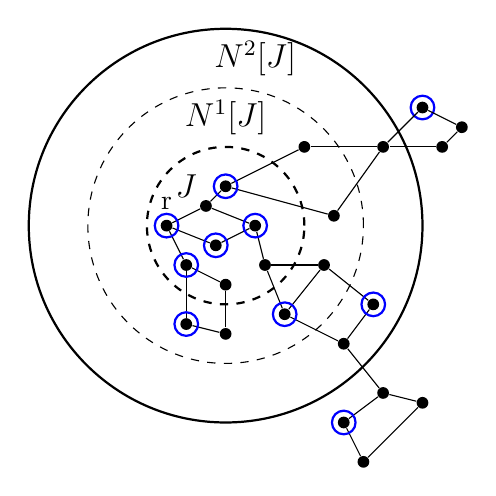
\begin{tikzpicture}[scale=0.5]
                \node[fill=black, circle, inner sep=1.5pt] (j01) at (0.75,0.5) {};
                \node[fill=black, circle, inner sep=1.5pt, label=above:r] (j02) at (-0.5,1) {};
                \node[fill=black, circle, inner sep=1.5pt] (j03) at (0.5,1.5) {};
                \node[fill=black, circle, inner sep=1.5pt] (j04) at (1.75,1) {};
        
                \node[fill=black, circle, inner sep=1.5pt] (j1) at (0,0) {};
                \node[fill=black, circle, inner sep=1.5pt] (j2) at (2,0) {};
                \node[fill=black, circle, inner sep=1.5pt] (j3) at (1,2) {};
                \node[fill=black, circle, inner sep=1.5pt] (j4) at (1,-0.5) {};
                
                % Draw N^1[J] vertices
        
                \node[fill=black, circle, inner sep=1.5pt] (n11) at (3.5,0) {};
                \node[fill=black, circle, inner sep=1.5pt] (n12) at (3.75,1.25) {};
                \node[fill=black, circle, inner sep=1.5pt] (n13) at (3,3) {};
                \node[fill=black, circle, inner sep=1.5pt] (n14) at (0,-1.5) {};
                \node[fill=black, circle, inner sep=1.5pt] (n15) at (1,-1.75) {};
                \node[fill=black, circle, inner sep=1.5pt] (n16) at (2.5,-1.25) {};
        
        
                % Draw N^2[J] vertices
                \node[fill=black, circle, inner sep=1.5pt] (n21) at (5, 3) {};
                \node[fill=black, circle, inner sep=1.5pt] (n22) at (4,-2) {};
                \node[fill=black, circle, inner sep=1.5pt] (n23) at (4.75,-1) {};
        
                % Draw vertices outside N^2[J]
                \node[fill=black, circle, inner sep=1.5pt] (n31) at (4, -4) {};
                \node[fill=black, circle, inner sep=1.5pt] (n32) at (5, -3.25) {};
                \node[fill=black, circle, inner sep=1.5pt] (n33) at (6, -3.5) {};
                \node[fill=black, circle, inner sep=1.5pt] (n34) at (4.5, -5) {};

                \node[fill=black, circle, inner sep=1.5pt] (new31) at (6, 4) {};
                \node[fill=black, circle, inner sep=1.5pt] (new32) at (6.5, 3) {};
                \node[fill=black, circle, inner sep=1.5pt] (new33) at (7, 3.5) {};
                
        
                % Draw edges inside J (induced subgraph)
                \draw (j01) -- (j02);
                \draw (j02) -- (j03);
                \draw (j03) -- (j04);
                \draw (j04) -- (j01);
        
                \draw (j4) -- (j1);

                \draw (j02) -- (j1);
                \draw (j04) -- (j2);
                \draw (j03) -- (j3);
                
                % Draw edges from J to N^1[J]
                \draw (j2) -- (n11);
                \draw (j2) -- (n16);
                \draw (j3) -- (n12);
                \draw (j1) -- (n14);
                \draw (j3) -- (n13);
                \draw (j4) -- (n15);
        
                % Draw edges inside N^1[J]
                \draw (n14) -- (n15);
                \draw (n16) -- (n11);
        
                % Draw edges between N^1[J] and N^2[J]
                \draw (n16) -- (n22);
                \draw (n11) -- (n23);
                \draw (n13) -- (n21);
                \draw (n12) -- (n21);
        
                % Draw edges between N^2[J] and N^2[J]
                \draw (n22) -- (n23);
        
                % Draw edges between N^2[J] and the other part of the graph
                \draw (n22) -- (n32);
        
                % Draw edges between the edges that are outside of N^2[J]
                \draw (n31) -- (n32);
                \draw (n32) -- (n33);
                \draw (n33) -- (n34);
                \draw (n34) -- (n31);
        
                % Draw the J circle
                \draw[dashed, thick] (1,1) circle [radius=2];
                \node at (0,2) {\large $J$};
        
                \draw[dashed] (1,1) circle [radius=3.5];
                \node at (1,3.75) {\large $N^1[J]$};
                
                % Draw the N^2[J] boundary as a larger circle
                \draw[thick] (1,1) circle [radius=5];
                \node at (1.75,5.25) {\large $N^2[J]$};
        
                % Draw vertices that are part of S_1
                \draw[blue, thick] (j01) circle(0.3);
                \draw[blue, thick] (j02) circle(0.3);
                \draw[blue, thick] (j04) circle(0.3);
        
                \draw[blue, thick] (j1) circle(0.3);
                \draw[blue, thick] (j3) circle(0.3);
                \draw[blue, thick] (n14) circle(0.3);
                \draw[blue, thick] (n16) circle(0.3);
                \draw[blue, thick] (n23) circle(0.3);
                \draw[blue, thick] (n31) circle(0.3);
                \draw[blue, thick] (new31) circle(0.3);

                \draw (n21) -- (new31);
                \draw (n21) -- (new32);
                \draw (new31) -- (new33);
                \draw (new32) -- (new33);
    \end{tikzpicture}
    \captionof{figure}{Sets $J \subseteq N^{1}_{G}[J] \subseteq N^{2}_{G}[J]$; Solution 
    $S_1$ in blue}
\end{minipage}
\hfill
\begin{minipage}{0.48\textwidth}
    \centering
    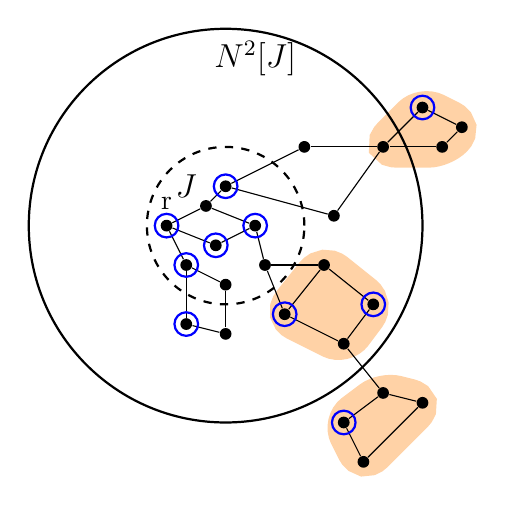
\begin{tikzpicture}[scale=0.5]
        \node[fill=black, circle, inner sep=1.5pt] (j01) at (0.75,0.5) {};
                \node[fill=black, circle, inner sep=1.5pt, label=above:r] (j02) at (-0.5,1) {};
                \node[fill=black, circle, inner sep=1.5pt] (j03) at (0.5,1.5) {};
                \node[fill=black, circle, inner sep=1.5pt] (j04) at (1.75,1) {};
    
                \node[fill=black, circle, inner sep=1.5pt] (j1) at (0,0) {};
                \node[fill=black, circle, inner sep=1.5pt] (j2) at (2,0) {};
                \node[fill=black, circle, inner sep=1.5pt] (j3) at (1,2) {};
                \node[fill=black, circle, inner sep=1.5pt] (j4) at (1,-0.5) {};
                
                % Draw N^1[J] vertices
    
                \node[fill=black, circle, inner sep=1.5pt] (n11) at (3.5,0) {};
                \node[fill=black, circle, inner sep=1.5pt] (n12) at (3.75,1.25) {};
                \node[fill=black, circle, inner sep=1.5pt] (n13) at (3,3) {};
                \node[fill=black, circle, inner sep=1.5pt] (n14) at (0,-1.5) {};
                \node[fill=black, circle, inner sep=1.5pt] (n15) at (1,-1.75) {};
                \node[fill=black, circle, inner sep=1.5pt] (n16) at (2.5,-1.25) {};
    
    
                % Draw N^2[J] vertices
                \node[fill=black, circle, inner sep=1.5pt] (n21) at (5, 3) {};
                \node[fill=black, circle, inner sep=1.5pt] (n22) at (4,-2) {};
                \node[fill=black, circle, inner sep=1.5pt] (n23) at (4.75,-1) {};
    
                % Draw vertices outside N^2[J]
                \node[fill=black, circle, inner sep=1.5pt] (n31) at (4, -4) {};
                \node[fill=black, circle, inner sep=1.5pt] (n32) at (5, -3.25) {};
                \node[fill=black, circle, inner sep=1.5pt] (n33) at (6, -3.5) {};
                \node[fill=black, circle, inner sep=1.5pt] (n34) at (4.5, -5) {};

                \node[fill=black, circle, inner sep=1.5pt] (new31) at (6, 4) {};
                \node[fill=black, circle, inner sep=1.5pt] (new32) at (6.5, 3) {};
                \node[fill=black, circle, inner sep=1.5pt] (new33) at (7, 3.5) {};
    
                % Draw edges inside J (induced subgraph)
                \draw (j01) -- (j02);
                \draw (j02) -- (j03);
                \draw (j03) -- (j04);
                \draw (j04) -- (j01);
    
                \draw (j4) -- (j1);

                \draw (j02) -- (j1);
                \draw (j04) -- (j2);
                \draw (j03) -- (j3);
                
                % Draw edges from J to N^1[J]
                \draw (j2) -- (n11);
                \draw (j2) -- (n16);
                \draw (j3) -- (n12);
                \draw (j1) -- (n14);
                \draw (j3) -- (n13);
                \draw (j4) -- (n15);
    
                % Draw edges inside N^1[J]
                \draw (n14) -- (n15);
                \draw (n16) -- (n11);
    
                % Draw edges between N^1[J] and N^2[J]
                \draw (n16) -- (n22);
                \draw (n11) -- (n23);
                \draw (n13) -- (n21);
                \draw (n12) -- (n21);
    
                % Draw edges between N^2[J] and N^2[J]
                \draw (n22) -- (n23);
    
                % Draw edges between N^2[J] and the other part of the graph
                \draw (n22) -- (n32);
    
                % Draw edges between the edges that are outside of N^2[J]
                \draw (n31) -- (n32);
                \draw (n32) -- (n33);
                \draw (n33) -- (n34);
                \draw (n34) -- (n31);

                \draw (n21) -- (new31);
                \draw (n21) -- (new32);
                \draw (new31) -- (new33);
                \draw (new32) -- (new33);
    
                % Draw the J circle
                \draw[dashed, thick] (1,1) circle [radius=2];
                \node at (0,2) {\large $J$};
    
                % Draw the N^2[J] boundary as a larger circle
                \draw[thick] (1,1) circle [radius=5];
                \node at (1.75,5.25) {\large $N^2[J]$};
    
                % Draw vertices that are part of S_1
                \draw[blue, thick] (j01) circle(0.3);
                \draw[blue, thick] (j02) circle(0.3);
                \draw[blue, thick] (j04) circle(0.3);
    
                \draw[blue, thick] (j1) circle(0.3);
                \draw[blue, thick] (j3) circle(0.3);
                \draw[blue, thick] (n14) circle(0.3);
                \draw[blue, thick] (n16) circle(0.3);
                \draw[blue, thick] (n23) circle(0.3);
                \draw[blue, thick] (n31) circle(0.3);
                \draw[blue, thick] (new31) circle(0.3);
    
                \begin{scope}[on background layer]   
                    \filldraw[orange!35,line width=15pt,rounded corners=5pt] (n31.center) -- (n32.center) -- (n33.center) -- (n34.center) -- cycle;
                \end{scope}
    
                \begin{scope}[on background layer]   
                    \filldraw[orange!35,line width=15pt,rounded corners=5pt] (n22.center) -- (n23.center) -- (n11.center) -- (n16.center) -- cycle;
                \end{scope}

                \begin{scope}[on background layer]   
                    \filldraw[orange!35,line width=15pt,rounded corners=5pt] (n21.center) -- (new31.center) -- (new33.center) -- (new32.center) -- cycle;
                \end{scope}
    \end{tikzpicture}
    \captionof{figure}{$\forall v \in \{v_1,v_2,v_3,v_4\}$, such that $v \in S_1$, it holds that 
    $v \notin J$}
\end{minipage}

\end{frame}

\begin{frame}{Case-distinction proof}
\centering

\begin{minipage}{0.48\textwidth}
    \centering
    \begin{tikzpicture}[scale=0.5]
        \node[fill=black, circle, inner sep=1.5pt] (j01) at (0.75,0.5) {};
                \node[fill=black, circle, inner sep=1.5pt, label=above:r] (j02) at (-0.5,1) {};
                \node[fill=black, circle, inner sep=1.5pt] (j03) at (0.5,1.5) {};
                \node[fill=black, circle, inner sep=1.5pt] (j04) at (1.75,1) {};
        
                \node[fill=black, circle, inner sep=1.5pt] (j1) at (0,0) {};
                \node[fill=black, circle, inner sep=1.5pt] (j2) at (2,0) {};
                \node[fill=black, circle, inner sep=1.5pt] (j3) at (1,2) {};
                \node[fill=black, circle, inner sep=1.5pt] (j4) at (1,-0.5) {};
                
                % Draw N^1[J] vertices
        
                \node[fill=black, circle, inner sep=1.5pt] (n11) at (3.5,0) {};
                \node[fill=black, circle, inner sep=1.5pt] (n12) at (3.75,1.25) {};
                \node[fill=black, circle, inner sep=1.5pt] (n13) at (3,3) {};
                \node[fill=black, circle, inner sep=1.5pt, label=below:$v_{1,4}$]  at (0,-1.5) {};
                \node[fill=black, circle, inner sep=1.5pt] (n15) at (1,-1.75) {};
                \node[fill=black, circle, inner sep=1.5pt] (n16) at (2.5,-1.25) {};
        
        
                % Draw N^2[J] vertices
                \node[fill=black, circle, inner sep=1.5pt] (n21) at (5, 3) {};
                \node[fill=black, circle, inner sep=1.5pt] (n22) at (4,-2) {};
                \node[fill=black, circle, inner sep=1.5pt] (n23) at (4.75,-1) {};
        
                % Draw vertices outside N^2[J]
                \node[fill=black, circle, inner sep=1.5pt] (n31) at (4, -4) {};
                \node[fill=black, circle, inner sep=1.5pt] (n32) at (5, -3.25) {};
                \node[fill=black, circle, inner sep=1.5pt] (n33) at (6, -3.5) {};
                \node[fill=black, circle, inner sep=1.5pt] (n34) at (4.5, -5) {};

                \node[fill=black, circle, inner sep=1.5pt] (new31) at (6, 4) {};
                \node[fill=black, circle, inner sep=1.5pt] (new32) at (6.5, 3) {};
                \node[fill=black, circle, inner sep=1.5pt] (new33) at (7, 3.5) {};

                % Draw edges inside J (induced subgraph)
                \draw (j01) -- (j02);
                \draw (j02) -- (j03);
                \draw (j03) -- (j04);
                \draw (j04) -- (j01);
        
                \draw (j4) -- (j1);

                \draw (j02) -- (j1);
                \draw (j04) -- (j2);
                \draw (j03) -- (j3);
                
                % Draw edges from J to N^1[J]
                \draw (j2) -- (n11);
                \draw (j2) -- (n16);
                \draw (j3) -- (n12);
                \draw (j1) -- (n14);
                \draw (j3) -- (n13);
                \draw (j4) -- (n15);
        
                % Draw edges inside N^1[J]
                \draw (n14) -- (n15);
                \draw (n16) -- (n11);
        
                % Draw edges between N^1[J] and N^2[J]
                \draw (n16) -- (n22);
                \draw (n11) -- (n23);
                \draw (n13) -- (n21);
                \draw (n12) -- (n21);
        
                % Draw edges between N^2[J] and N^2[J]
                \draw (n22) -- (n23);
        
                % Draw edges between N^2[J] and the other part of the graph
                \draw (n22) -- (n32);
        
                % Draw edges between the edges that are outside of N^2[J]
                \draw (n31) -- (n32);
                \draw (n32) -- (n33);
                \draw (n33) -- (n34);
                \draw (n34) -- (n31);

                \draw (n21) -- (new31);
                \draw (n21) -- (new32);
                \draw (new31) -- (new33);
                \draw (new32) -- (new33);
        
                % Draw the J circle
                \draw[dashed, thick] (1,1) circle [radius=2];
                \node at (0,2) {\large $J$};
        
                % Draw the N^2[J] boundary as a larger circle
                \draw[thick] (1,1) circle [radius=5];
                \node at (1.75,5.25) {\large $N^2[J]$};
        
                % Draw vertices that are part of S_1
                \draw[blue, thick] (j01) circle(0.3);
                \draw[blue, thick] (j02) circle(0.3);
                \draw[blue, thick] (j04) circle(0.3);
        
                \draw[blue, thick] (j1) circle(0.3);
                \draw[blue, thick] (j3) circle(0.3);
                \draw[blue, thick] (n14) circle(0.3);
                \draw[blue, thick] (n16) circle(0.3);
                \draw[blue, thick] (n23) circle(0.3);
                \draw[blue, thick] (n31) circle(0.3);
                \draw[blue, thick] (new31) circle(0.3);
    
                \begin{scope}[on background layer]   
                    \filldraw[orange!35,line width=15pt,rounded corners=5pt] (j1.center) -- (n14.center) -- (n15.center) -- (j4.center) -- cycle;
                \end{scope}
    \end{tikzpicture}
    \captionof{figure}{$\exists v \in \{v_1,v_2,v_3,v_4\}$, such that $v \in S_1$: $v \in J$}
\end{minipage}
\hfill
\begin{minipage}{0.48\textwidth}
    \centering
    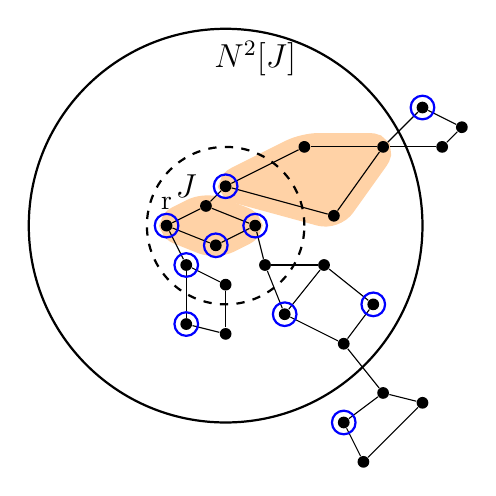
\begin{tikzpicture}[scale=0.5]
        %Draw J vertices
                \node[fill=black, circle, inner sep=1.5pt] (j01) at (0.75,0.5) {};
                \node[fill=black, circle, inner sep=1.5pt, label=above:r] (j02) at (-0.5,1) {};
                \node[fill=black, circle, inner sep=1.5pt] (j03) at (0.5,1.5) {};
                \node[fill=black, circle, inner sep=1.5pt] (j04) at (1.75,1) {};
    
                \node[fill=black, circle, inner sep=1.5pt] (j1) at (0,0) {};
                \node[fill=black, circle, inner sep=1.5pt] (j2) at (2,0) {};
                \node[fill=black, circle, inner sep=1.5pt] (j3) at (1,2) {};
                \node[fill=black, circle, inner sep=1.5pt] (j4) at (1,-0.5) {};
                
                % Draw N^1[J] vertices
    
                \node[fill=black, circle, inner sep=1.5pt] (n11) at (3.5,0) {};
                \node[fill=black, circle, inner sep=1.5pt] (n12) at (3.75,1.25) {};
                \node[fill=black, circle, inner sep=1.5pt] (n13) at (3,3) {};
                \node[fill=black, circle, inner sep=1.5pt] (n14) at (0,-1.5) {};
                \node[fill=black, circle, inner sep=1.5pt] (n15) at (1,-1.75) {};
                \node[fill=black, circle, inner sep=1.5pt] (n16) at (2.5,-1.25) {};
    
    
                % Draw N^2[J] vertices
                \node[fill=black, circle, inner sep=1.5pt] (n21) at (5, 3) {};
                \node[fill=black, circle, inner sep=1.5pt] (n22) at (4,-2) {};
                \node[fill=black, circle, inner sep=1.5pt] (n23) at (4.75,-1) {};
    
                % Draw vertices outside N^2[J]
                \node[fill=black, circle, inner sep=1.5pt] (n31) at (4, -4) {};
                \node[fill=black, circle, inner sep=1.5pt] (n32) at (5, -3.25) {};
                \node[fill=black, circle, inner sep=1.5pt] (n33) at (6, -3.5) {};
                \node[fill=black, circle, inner sep=1.5pt] (n34) at (4.5, -5) {};

                \node[fill=black, circle, inner sep=1.5pt] (new31) at (6, 4) {};
                \node[fill=black, circle, inner sep=1.5pt] (new32) at (6.5, 3) {};
                \node[fill=black, circle, inner sep=1.5pt] (new33) at (7, 3.5) {};
    
                % Draw edges inside J (induced subgraph)
                \draw (j01) -- (j02);
                \draw (j02) -- (j03);
                \draw (j03) -- (j04);
                \draw (j04) -- (j01);
    
                \draw (j4) -- (j1);

                \draw (j02) -- (j1);
                \draw (j04) -- (j2);
                \draw (j03) -- (j3);
                
                % Draw edges from J to N^1[J]
                \draw (j2) -- (n11);
                \draw (j2) -- (n16);
                \draw (j3) -- (n12);
                \draw (j1) -- (n14);
                \draw (j3) -- (n13);
                \draw (j4) -- (n15);
    
                % Draw edges inside N^1[J]
                \draw (n14) -- (n15);
                \draw (n16) -- (n11);
    
                % Draw edges between N^1[J] and N^2[J]
                \draw (n16) -- (n22);
                \draw (n11) -- (n23);
                \draw (n13) -- (n21);
                \draw (n12) -- (n21);
    
                % Draw edges between N^2[J] and N^2[J]
                \draw (n22) -- (n23);
    
                % Draw edges between N^2[J] and the other part of the graph
                \draw (n22) -- (n32);
    
                % Draw edges between the edges that are outside of N^2[J]
                \draw (n31) -- (n32);
                \draw (n32) -- (n33);
                \draw (n33) -- (n34);
                \draw (n34) -- (n31);

                \draw (n21) -- (new31);
                \draw (n21) -- (new32);
                \draw (new31) -- (new33);
                \draw (new32) -- (new33);
    
                % Draw the J circle
                \draw[dashed, thick] (1,1) circle [radius=2];
                \node at (0,2) {\large $J$};
    
                % Draw the N^2[J] boundary as a larger circle
                \draw[thick] (1,1) circle [radius=5];
                \node at (1.75,5.25) {\large $N^2[J]$};
    
                % Draw vertices that are part of S_1
                \draw[blue, thick] (j01) circle(0.3);
                \draw[blue, thick] (j02) circle(0.3);
                \draw[blue, thick] (j04) circle(0.3);
    
                \draw[blue, thick] (j1) circle(0.3);
                \draw[blue, thick] (j3) circle(0.3);
                \draw[blue, thick] (n14) circle(0.3);
                \draw[blue, thick] (n16) circle(0.3);
                \draw[blue, thick] (n23) circle(0.3);
                \draw[blue, thick] (n31) circle(0.3);
                \draw[blue, thick] (new31) circle(0.3);
    
                \begin{scope}[on background layer]   
                    \filldraw[orange!35,line width=10pt,rounded corners=5pt] (j01.center) -- (j02.center) -- (j03.center) -- (j04.center) -- cycle;
                \end{scope}
    
                \begin{scope}[on background layer]   
                    \filldraw[orange!35,line width=10pt,rounded corners=5pt] (j3.center) -- (n12.center) -- (n21.center) -- (n13.center) -- cycle;
                \end{scope}
    
    \end{tikzpicture}
    \captionof{figure}{$\forall v \in \{v_1,v_2,v_3,v_4\}$, such that $v \in S_1$: $v \in J$}
\end{minipage}

\end{frame}

\begin{frame}{Meta-Theorem for Minor-Closed Graph Classes}

\begin{theorem}[Meta-Theorem for Minor-Closed Graph Classes]
Let $\mathcal{G}$ be a minor-closed graph class whose local treewidth is bounded by $g(r) = \lambda \cdot r$, for fixed $\lambda \in \mathbb{R}$ and $r \in \mathbb{N}$.

Let $\Pi$ be a vertex-minimization problem such that:
\begin{enumerate}
    \item $\Pi$ is guessable.
    \item $\Pi$ is m-stitchable.
    \item There exists an algorithm $A_\Pi$ that solves $\Pi$-$m$-stitching in time 
    $f(t) \cdot |V(G)|^{\mathcal{O}(1)}$, where $t = \tw(G[N_G^m(J)])$ and $f$ is computable.
\end{enumerate}

Then, for each $\epsilon > 0$, there exists a $(1 + \epsilon)$-certified algorithm for $\Pi$ 
running in time $f(\lambda \cdot m / \epsilon) \cdot |V(G)|^{\mathcal{O}(1)}$ on any input 
$(G, w : V(G) \to \mathbb{N})$, with $G \in \mathcal{G}$ and polynomially-bounded weights.
\end{theorem}

\end{frame}

\begin{frame}[fragile]{{$(1+\epsilon)$}-Certified Algorithm for FVS-4CL}
  \begin{algorithm}[H]
    \caption{$(1+\epsilon)$-Certified algorithm for FVS-4CL}
    \begin{algorithmic}[1]
    \REQUIRE Vertex-weighted planar graph $(G, w:V(G) \to \mathbb{N})$, $\epsilon > 0$
    \ENSURE A vertex set $S^* \subseteq V(G)$ and a $(1+\epsilon)$-perturbation $w'$ of $w$ such that $S^*$ is optimal for FVS-4CL on $(G, w')$
    \STATE $\kappa \leftarrow \left\lceil \frac{2m}{\epsilon} \right\rceil + 2m$, where $m \leftarrow 2$
    \STATE Let $S^*$ be a feasible solution (FVS-4CL is guessable)
    \STATE Perform BFS from an arbitrary vertex $r$
    \WHILE{there exists a subgraph $J_{\kappa-2m}$ of width $\kappa - 2m$ such that \\ \hspace{1.5em} $w_A((G,w), S^*, J_{\kappa-2m}) < w(S^*)$}
        \STATE $S^* \leftarrow A((G,w), S^*, J_{\kappa-2m})$
    \ENDWHILE
    \STATE Define $w': V(G) \rightarrow \mathbb{R}^+$ by:
    \[
    w'(x) = 
    \begin{cases}
    w(x) & \text{if } x \in S^* \\
    (1 + \epsilon)w(x) & \text{otherwise}
    \end{cases}
    \]
    \RETURN $(S^*, w')$
    \end{algorithmic}
  \end{algorithm}
\end{frame}


\section{Conclusion}

\begin{frame}{Summary of Contributions}
\begin{itemize}
    \item Applied \textbf{Baker's technique} to establish an 
    \textbf{EPTAS for the FVS-BCL and FVS-4CL problems} in planar graphs.
    
    \item Proved that the \textbf{FVS-4CL problem is tractable} via 
    \textbf{dynamic programming over nice tree decompositions}, and that the 
    \textbf{FVS-BCL problem is tractable} via a formulation in 
    \textbf{monadic second-order logic (MSOL)}.
    
    \item Designed an algorithm for computing 
    \textbf{(1 + $\varepsilon$)-certified solutions} for both problems.

\end{itemize}
\end{frame}


\begin{frame}{Future Work}
  \begin{itemize}
    \item Extend the DP algorithm over nice tree decompositions to FVS-BCL
    \item Improve the current algorithm that has a running time of 
    $2^{\mathcal{O}(\tw^2)} \cdot n^{\mathcal{O}(1)}$
    \begin{itemize} 
    \item Cut \& Count technique, which obtained a 
    $3^{\mathcal{O}(\tw)} \cdot n^{\mathcal{O}(1)}$ randomized algorithm
    \textbf{(Cygan et al., 2011)}  

    \item Deterministic 
    $2^{\mathcal{O}(\tw)} \cdot n^{\mathcal{O}(1)}$ rank-based approach
    \textbf{(Bodlaender et al., 2015)}

    \end{itemize}
    \item  Improve the certified algorithm for FVS-BCL. 
    In particular, it would be valuable to develop an approach that eliminates the current 
    reliance on the polynomially-bounded weights constraint
  \end{itemize}
\end{frame}

\begin{frame}
  \centering
  \Huge Thank you!\\
  \vspace{0.5cm}
  \Large Questions?
\end{frame}

\end{document}
